\documentclass[journal,onecolumn,draftclsnofoot,12pt]{IEEEtran}
\usepackage{cite}
\usepackage{amsmath,amssymb}
\usepackage{graphicx}
\usepackage{booktabs}
\usepackage{multirow}
\usepackage{algorithm}
\usepackage{algpseudocode}
\usepackage{tikz}
\usetikzlibrary{positioning,arrows.meta,fit}
\usepackage{setspace}
\usepackage[hidelinks]{hyperref}
\renewcommand{\algorithmicrequire}{\textbf{Input:}}
\renewcommand{\algorithmicensure}{\textbf{Output:}}
\newcommand{\pmv}[2]{#1{\scriptsize$\pm$#2}}

\begin{document}
\doublespacing

\title{EASFL: Energy-Aware, Poisoning-Resilient Federated Learning for Anomaly Detection and Lifetime Extension in Wireless Sensor Networks}

\author{Shiva~Kumar~V
and~Choupiri~Shivakeshi
\thanks{Shiva Kumar V (corresponding author) and Choupiri Shivakeshi are with the Department of Computer Science and Engineering, Kishkinda University, Ballari, Karnataka, India (e-mail: shivakumar@kishkindauniversity.edu.in; shivakeshic@kishkindauniversity.edu.in).}}

\markboth{IEEE Transactions on Green Communications and Networking}{Shiva Kumar V and Shivakeshi: EASFL for Anomaly Detection in WSNs}

\maketitle

\begin{abstract}
Federated learning (FL) keeps raw sensor data on the nodes of a wireless sensor network (WSN), but repeatedly exchanging model updates over low-power radios can drain batteries faster than shipping the raw data itself. We present EASFL, a cluster-based FL framework for on-node anomaly detection that treats energy as a first-class constraint. EASFL combines (i) cluster-head selection scored on residual energy, distance to the sink and local connectivity; (ii) per-cluster participant selection that rests low-energy and quarantined nodes; (iii) top-$k$ sparsified, 8-bit quantized updates with error feedback; (iv) two-tier robust aggregation with norm and direction filtering, trimmed means and a reputation-based quarantine; and (v) zero-communication on-node personalization through local fine-tuning and threshold calibration. In a 100-node simulation with the first-order radio model and a fully specified synthetic sensing workload with four realistic fault types, EASFL reduces over-the-air traffic by $13\times$ and energy use by $3\times$ relative to hierarchical FedAvg, delays the first node death from round 35 to round 547, and keeps all nodes alive at round 200, where it attains a network-level F1-score of 0.82 against 0.26 for hierarchical FedAvg and 0.70 for centralized learning. Personalization closes the non-IID accuracy gap (per-node F1 0.71 $\rightarrow$ 0.82, above the 0.78 of a centralized model), and the defence keeps F1 within 0.07 of its clean value against four poisoning attacks with up to 20\% malicious nodes. The conclusions hold across sweeps of data heterogeneity, fault magnitude, anomaly rate and packet loss.
\end{abstract}

\begin{IEEEkeywords}
Wireless sensor networks, federated learning, anomaly detection, energy efficiency, network lifetime, clustering, model poisoning, non-IID data, personalization.
\end{IEEEkeywords}

\section{Introduction}
\IEEEPARstart{W}{ireless} sensor networks (WSNs) underpin environmental, structural and industrial monitoring in the Internet of Things (IoT). Their readings are routinely corrupted by spikes, stuck-at values, drifts and noise bursts caused by failing hardware, depleted batteries, environmental extremes or tampering~\cite{ni2009,sharma2010}, and detecting such anomalies close to the source is essential for data quality and security~\cite{rajasegarar2008}. The conventional approach forwards raw readings to a base station (BS) for centralized learning. This exposes potentially sensitive data, adds latency and, crucially for battery-powered nodes, spends scarce energy on bulk transmission.

Federated learning (FL)~\cite{mcmahan2017,kairouz2021} offers an alternative: nodes train locally and share only model updates. FL has been applied to IoT anomaly and intrusion detection~\cite{nguyen2019diot,mothukuri2022}, but most work assumes edge devices with stable power and connectivity~\cite{lim2020}. In a WSN, three problems remain. First, \emph{communication energy}: every round moves a full model from every participant, so naive FL can exhaust the network faster than centralized collection (Section~\ref{sec:results}). Second, \emph{heterogeneity}: each node sees its own environment and fault mix, so data are non-IID and a single global model under-fits individual nodes~\cite{zhao2018,hsu2019}. Third, \emph{trust}: nodes are physically exposed, and a few compromised nodes can poison the shared model~\cite{blanchard2017,fang2020}. Existing studies usually address one of these in isolation, and few report how learning choices translate into network lifetime.

This paper proposes EASFL, an energy-aware, poisoning-resilient FL framework that addresses all three jointly within the clustered architecture already standard in WSNs~\cite{heinzelman2002,younis2004,abbasi2007}. Our contributions are:
\begin{enumerate}
\item A cluster-based FL protocol whose every component (head selection, participant selection, update compression, aggregation) is chosen to reduce radio energy, with an explicit bit-level cost model.
\item A two-tier robust aggregation scheme with reputation-based quarantine that requires no trusted root dataset, and a zero-communication on-node personalization step that resolves the non-IID accuracy gap.
\item A reproducible evaluation with energy-coupled detection metrics, including a \emph{network-level} F1-score in which nodes that have exhausted their batteries raise no alarms, ablations, four attack models against three robust-aggregation baselines, and sensitivity analyses of the synthetic workload. All code and seeds are released.
\end{enumerate}

\section{Related Work}
\textit{Energy-efficient clustering.} LEACH~\cite{heinzelman2002} rotates cluster heads (CHs) randomly to spread load, and HEED~\cite{younis2004} uses residual energy and communication cost; see~\cite{abbasi2007} for a survey. These protocols target data gathering; EASFL reuses their structure but adapts head and participant selection to the FL workload.

\textit{Communication-efficient and resource-aware FL.} Sparsification with error feedback~\cite{lin2018dgc,stich2018} and sparse ternary compression~\cite{sattler2020} reduce upload volume, client selection accounts for heterogeneous resources~\cite{nishio2019}, hierarchical client--edge--cloud aggregation cuts long-haul traffic~\cite{liu2020hfl}, and adaptive aggregation frequency trades computation for communication~\cite{wang2019adaptive}. These works measure cost in bytes or wall-clock time; we measure it in joules under a WSN radio model and report its effect on node deaths.

\textit{Robust FL and heterogeneity.} Byzantine-robust rules include Krum~\cite{blanchard2017}, coordinate-wise median and trimmed mean~\cite{yin2018}, and FLTrust, which requires a clean root dataset at the server~\cite{cao2021}. Adaptive attacks~\cite{fang2020} and backdoors~\cite{bagdasaryan2020} show that no single rule suffices. For non-IID data, proximal regularization (FedProx)~\cite{li2020fedprox} and personalization~\cite{arivazhagan2019,tan2023} are common. Cryptographic secure aggregation~\cite{bonawitz2017} protects update confidentiality but not integrity and is orthogonal to our design.

\textit{FL for IoT anomaly detection.} D\"IoT~\cite{nguyen2019diot} and~\cite{mothukuri2022} detect compromised IoT devices with FL, but target gateways or mains-powered devices and do not model radio energy or lifetime. To our knowledge, EASFL is the first framework to evaluate head selection, participant selection, compression, robust aggregation and personalization together under a WSN energy model with lifetime and network-level detection as joint outcomes.

\section{System Model}\label{sec:model}
\subsection{Network and Energy Model}
$N$ static nodes are deployed uniformly in an $L\times L$ field with a BS outside the field. Node $i$ starts with heterogeneous energy $E_i^0\sim\mathcal{U}[0.25,0.75]$\,J. Time is divided into rounds; in each round clusters are formed, members exchange data or updates with their CH, and CHs communicate with the BS over a single hop. We adopt the first-order radio model~\cite{heinzelman2002}: transmitting $\ell$ bits over distance $d$ costs
\begin{equation}
E_{\mathrm{tx}}(\ell,d)=\begin{cases}\ell E_{\mathrm{elec}}+\ell\varepsilon_{\mathrm{fs}}d^{2}, & d<d_0,\\ \ell E_{\mathrm{elec}}+\ell\varepsilon_{\mathrm{mp}}d^{4}, & d\ge d_0,\end{cases}
\end{equation}
and $E_{\mathrm{rx}}(\ell)=\ell E_{\mathrm{elec}}$,
with $d_0=\sqrt{\varepsilon_{\mathrm{fs}}/\varepsilon_{\mathrm{mp}}}\approx 87.7$\,m. CHs spend $E_{\mathrm{DA}}$ per bit to aggregate. Local training costs $e_s$ joules per sample-pass, so a round of $n_s$ samples costs $n_se_s$. Every packet carries a 200-bit header, and cluster advertisement and join messages are 200-bit control packets. A packet is lost independently with probability $p_\ell$. A node dies when its energy reaches zero. Lifetime is reported as the rounds until the first node dies (FND), half the nodes die (HND) and 90\% die (LND).

\subsection{Sensing Workload and Fault Model}
Because labelled fault data from real deployments are scarce and their ground truth is uncertain~\cite{sharma2010}, we use a fully specified synthetic workload that reproduces the structure of indoor/outdoor environmental WSNs. Node $i$ samples temperature, humidity, light and supply voltage once per minute:
\begin{align}
T_i(t)&=\bar T_i+A_i\sin(2\pi t/1440+\phi_i)+n_T,\nonumber\\
H_i(t)&=\bar H_i-1.5\,(T_i(t)-\bar T_i)+n_H,\\
L_i(t)&=\bar L_i\max\!\big(0,\sin(2\pi t/1440+\phi_i)\big)+n_L,\nonumber\\
V_i(t)&=2.9-10^{-5}t+n_V,\nonumber
\end{align}
with $\bar T_i\sim\mathcal{U}[18,30]^\circ$C, $A_i\sim\mathcal{U}[1,5]$, $\bar H_i\sim\mathcal{U}[30,60]\%$, $\bar L_i\sim\mathcal{U}[100,600]$\,lux and zero-mean Gaussian noise with standard deviations $\kappa_i(0.15,0.5,10,0.005)$, $\kappa_i\sim\mathcal{U}[0.7,1.6]$; 40\% of nodes are outdoor, with three-fold light noise. Readings are grouped into windows of $W=10$ samples. Each window of node $i$ is anomalous with a node-specific rate
\[\lambda_i=\mathrm{clip}\big(\mathrm{LogNormal}(\ln 0.07,0.8),\,0.01,\,0.30\big),\]
and the fault type is drawn from a node-specific mixture $\boldsymbol\pi_i\sim\mathrm{Dir}(\alpha\mathbf{1})$, $\alpha=0.5$, over the four types catalogued in~\cite{ni2009,sharma2010}: \emph{spike} (one sample offset), \emph{stuck-at} (a channel frozen), \emph{drift} (a linear ramp) and \emph{noise burst}. The fault affects one random channel with magnitude $a\sim\mathcal{U}[3,8]$ times that channel's noise level. The Dirichlet prior makes the label and fault distributions non-IID across nodes, with $\alpha$ controlling the degree~\cite{hsu2019}.

From each window we extract, per channel, the standard deviation, range, maximum absolute first difference, absolute linear-trend slope, maximum absolute residual after detrending and fraction of repeated samples, giving 24 features. Features are scaled by the nominal channel noise, log-compressed and standardized with network-wide means and variances; these 48 scalars are obtained once at deployment by aggregating per-node sums and sums of squares, at a cost comparable to a single model update. Each node holds 200 training windows and is tested on the following 100 windows.

\subsection{Detector and Threat Model}
Every scheme uses the same detector, a 24--16--1 multilayer perceptron with ReLU hidden units and a sigmoid output ($P=417$ parameters), trained with class-weighted binary cross-entropy (positive weight 4) by mini-batch SGD. In FL rounds, each participant runs one local epoch on up to 150 windows (learning rate 0.15, batch 16) and reports its update $\Delta_i=w_i-w$.

A fraction $m$ of nodes is compromised at deployment. Compromised nodes follow the protocol but corrupt their own updates using one of four attacks: \emph{scaled sign flip} ($-4\Delta_i$); \emph{stealth sign flip} ($-\Delta_i$, which preserves the norm); \emph{label flip} (training on inverted labels); and \emph{Gaussian} (random direction with twice the honest norm). CHs are assumed to aggregate honestly; adversarial CHs are left for future work.

\section{The EASFL Framework}\label{sec:method}
Fig.~\ref{fig:arch} and Algorithm~\ref{alg:easfl} summarize one EASFL round.

\begin{figure}[t]
\centering
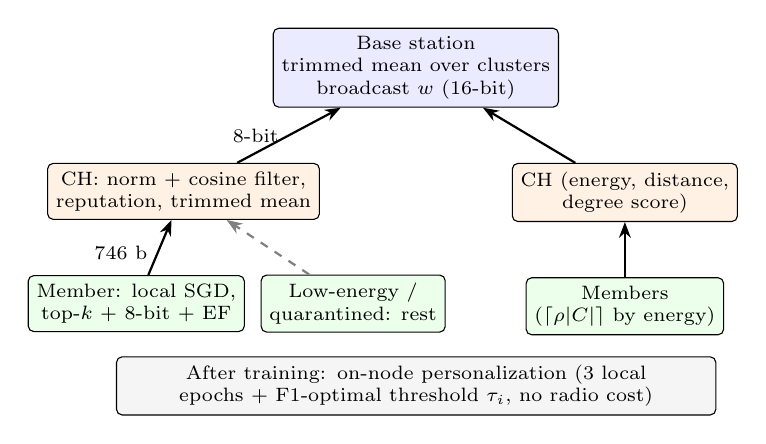
\begin{tikzpicture}[font=\scriptsize, node distance=3mm,
 box/.style={draw, rounded corners=2pt, align=center, inner sep=3pt, minimum height=6mm},
 arr/.style={-{Stealth[length=2mm]}, thick}]
\node[box, fill=blue!8] (bs) {Base station\\ trimmed mean over clusters\\ broadcast $w$ (16-bit)};
\node[box, fill=orange!10, below left=7mm and -6mm of bs] (ch1) {CH: norm + cosine filter,\\ reputation, trimmed mean};
\node[box, fill=orange!10, below right=7mm and -6mm of bs] (ch2) {CH (energy, distance,\\ degree score)};
\node[box, fill=green!8, below=7mm of ch1, xshift=-6mm] (m1) {Member: local SGD,\\ top-$k$ + 8-bit + EF};
\node[box, fill=green!8, right=2mm of m1] (m2) {Low-energy /\\ quarantined: rest};
\node[box, fill=green!8, below=7mm of ch2] (m3) {Members\\ ($\lceil\rho|C|\rceil$ by energy)};
\draw[arr] (m1) -- node[left, pos=0.4]{746 b} (ch1);
\draw[arr, dashed, gray] (m2) -- (ch1);
\draw[arr] (m3) -- (ch2);
\draw[arr] (ch1) -- node[left]{8-bit} (bs);
\draw[arr] (ch2) -- (bs);
\node[box, fill=gray!8, below=3mm of m2, xshift=8mm, text width=7.4cm] (p) {After training: on-node personalization (3 local epochs + F1-optimal threshold $\tau_i$, no radio cost)};
\end{tikzpicture}
\caption{EASFL round structure. Only selected members train and upload compressed updates; CHs filter and aggregate; the BS aggregates clusters robustly and broadcasts the model.}
\label{fig:arch}
\end{figure}

\subsection{Energy-Aware Cluster-Head Selection}
Let $\mathcal{A}$ be the set of alive nodes and $k=\mathrm{round}(p|\mathcal{A}|)$ with $p=0.1$. Each alive node receives the score
\begin{equation}
S_i=\big(0.5\,\hat E_i+0.3\,\hat D_i+0.2\,\hat G_i\big)\,\mathbf{1}[i\notin\mathcal{Q}],
\end{equation}
where $\hat E_i=E_i/\max_j E_j$ is normalized residual energy, $\hat D_i=1-(d_i-d_{\min})/(d_{\max}-d_{\min})$ rewards proximity to the BS, $\hat G_i$ is the normalized number of neighbours within 25\,m, and $\mathcal{Q}$ is the set of quarantined nodes. CHs are chosen greedily in decreasing $S_i$ subject to a minimum separation of 20\,m, which spreads clusters spatially. Each member joins its nearest CH. Unlike LEACH's randomized rotation, this keeps the energetically expensive CH role away from weak nodes.

\subsection{Energy-Aware Participant Selection}
Within cluster $C$, only nodes with $E_i>E_{\min}=0.025$\,J that are not quarantined are eligible, and the $\lceil\rho|C|\rceil$ eligible members with the highest residual energy participate ($\rho=0.5$). The others skip training and uploading but still receive the global model, so they keep detecting with the latest model.

\subsection{Compressed Updates}
Participants upload a sparsified, quantized update with error feedback~\cite{stich2018,lin2018dgc}. With residual memory $r_i$ (initially zero), node $i$ forms $v_i=\Delta_i+r_i$, keeps the $K=\lceil0.1P\rceil=42$ entries of largest magnitude, quantizes them uniformly to 8 bits with scale $s=\max|v_{i,k}|/127$, sends the result $q_i$ and sets $r_i\leftarrow v_i-q_i$. An upload thus takes $K(8+\lceil\log_2P\rceil)+32=746$ bits instead of $32P=13{,}344$ (17.9$\times$ smaller). CHs send dense 8-bit aggregates to the BS (3,368 bits, 4$\times$ smaller) and the BS broadcasts the model in 16-bit precision (6,672 bits).

\subsection{Two-Tier Robust Aggregation with Quarantine}
At CH $c$, let $U=\{u_i\}$ be the received (decoded) updates and $\tilde u=\mathrm{med}(U)$ their coordinate-wise median. Update $u_i$ is flagged if
\begin{equation}
\|u_i\|>3\,\mathrm{med}_j\|u_j\|\quad\text{or}\quad\cos(u_i,\tilde u)<0 .
\end{equation}
Each node keeps a suspicion score $f_i\leftarrow0.7f_i+\mathbf{1}[\text{flagged}]$; when $f_i>1.5$ (roughly two flags in three rounds) the node is quarantined for 20 rounds, during which it is excluded from participation and from CH candidacy. Unflagged updates are combined with a coordinate-wise trimmed mean (trim ratio 0.2), or the median if fewer than five remain~\cite{yin2018}. The BS combines cluster aggregates with a trimmed mean (ratio 0.1) when at least five arrive, and a sample-weighted mean otherwise. No trusted root dataset is needed, unlike~\cite{cao2021}.

\subsection{On-Node Personalization}
Non-IID fault mixes and rates make a single decision rule sub-optimal for every node. After federated training, each node fine-tunes the received model for three epochs on its own windows (learning rate 0.05) and selects the decision threshold $\tau_i$ that maximizes F1 on its training windows, in the spirit of personalized FL~\cite{arivazhagan2019,tan2023}. This step costs about 600 sample-passes ($\approx1.2$\,mJ, the training energy of four FL rounds) and no radio traffic.

\begin{algorithm}[t]
\caption{One EASFL round}\label{alg:easfl}
\begin{algorithmic}[1]
\Require global model $w$, residual energies $\{E_i\}$, quarantine set $\mathcal{Q}$
\State Select CHs by score $S_i$ with 20\,m separation; members join nearest CH
\For{each cluster $C$ with head $c$}
 \State $\mathcal{P}_C\gets$ top-$\lceil\rho|C|\rceil$ by $E_i$ among $\{i\in C: E_i>E_{\min}, i\notin\mathcal{Q}\}$
 \For{$i\in\mathcal{P}_C$} \Comment{in parallel}
   \State $\Delta_i\gets\mathrm{SGD}(w,\mathcal{D}_i)-w$; \ $v_i\gets\Delta_i+r_i$
   \State $q_i\gets Q_8(\mathrm{Top}_K(v_i))$; \ $r_i\gets v_i-q_i$; send $q_i$ to $c$
 \EndFor
 \State $c$: flag by norm/cosine, update $f_i$ and $\mathcal{Q}$, $a_C\gets\mathrm{TrMean}_{0.2}$(unflagged)
 \State $c$: send $Q_8(a_C)$ to BS
\EndFor
\State BS: $w\gets w+\mathrm{TrMean}_{0.1}(\{a_C\})$; broadcast $Q_{16}(w)$
\Ensure updated $w$; after training, each node personalizes ($w_i,\tau_i$)
\end{algorithmic}
\end{algorithm}

\section{Experimental Setup}\label{sec:setup}
Table~\ref{tab:params} lists the parameters. All results are means $\pm$ standard deviations over five seeds; each seed fixes the deployment, energies, attackers and data, so all schemes see identical conditions. Learning runs last 200 rounds; lifetime runs, which use the same energy accounting, continue until all nodes die (at most 4,000 rounds). The simulator is a round-based Python implementation of the model in Section~\ref{sec:model}; it abstracts the MAC layer and assumes perfect scheduling inside clusters.

\begin{table}[t]
\caption{Simulation Parameters}\label{tab:params}
\centering\scriptsize
\begin{tabular}{@{}ll@{}}
\toprule
Parameter & Value\\
\midrule
Nodes, field, BS position & 100; $100\times100$\,m; (50, 175)\,m\\
Initial energy & $\mathcal{U}[0.25,0.75]$\,J\\
$E_{\mathrm{elec}}$, $E_{\mathrm{DA}}$ & 50\,nJ/bit, 5\,nJ/bit\\
$\varepsilon_{\mathrm{fs}}$, $\varepsilon_{\mathrm{mp}}$ & 10\,pJ/bit/m$^2$, 0.0013\,pJ/bit/m$^4$\\
Training energy $e_s$ & 2\,$\mu$J per sample-pass\\
Header / control packet & 200 / 200 bits\\
CH fraction $p$; participation $\rho$ & 0.1; 0.5\\
Packet loss $p_\ell$ & 0.05 (swept 0--0.3)\\
Model & MLP 24--16--1, $P=417$\\
Local training & 1 epoch, $\le$150 windows, lr 0.15, batch 16\\
Compression & top-10\% (K=42), 8-bit, error feedback\\
Payloads (bits) & FedAvg 13,344; EASFL 746 up,\\
 & 3,368 CH$\to$BS, 6,672 down\\
Centralized raw data & 60 samples $\times$ 4 ch.\ $\times$ 16 bits per node-round\\
Rounds; seeds & 200 (learning), $\le$4000 (lifetime); 5\\
\bottomrule
\end{tabular}
\end{table}

\textit{Baselines.} \emph{Centralized} (CL): nodes send raw 16-bit samples through LEACH clusters to the BS, which trains the same MLP for 30 epochs on all data. \emph{Local}: each node trains its own MLP for 30 epochs without communication. \emph{FedAvg-flat}: all alive nodes train and send full-precision updates directly to the BS~\cite{mcmahan2017}. \emph{FedAvg-LEACH}: hierarchical FedAvg~\cite{liu2020hfl} over LEACH clusters with full-precision updates. For robustness we also equip FedAvg-LEACH with coordinate-wise \emph{median}, \emph{trimmed mean} (ratio 0.2)~\cite{yin2018} and \emph{Krum} ($f=0.2n$)~\cite{blanchard2017}, applied at both CH and BS.

\textit{Metrics.} Detection: accuracy, precision, recall, F1, false-positive rate (FPR) and AUC over all test windows of all nodes, for the global model (threshold 0.5) and after personalization. Because a depleted node cannot raise alarms, we also report \emph{network-level} F1 at round 200, where every window of a dead node is scored as normal. Efficiency: over-the-air uplink traffic, energy consumed in the first 200 rounds ($E_{200}$), and FND/HND/LND.

\section{Results}\label{sec:results}
\subsection{Detection, Traffic and Energy}
Table~\ref{tab:main} gives the main comparison. Without personalization, the hierarchical FL schemes reach a per-node F1 of about 0.71, below centralized learning (0.78) but above purely local models (0.69). FedAvg-flat is worse (0.59) because its participants die quickly and the model degrades after round 120 (Fig.~\ref{fig:conv}). EASFL matches FedAvg-LEACH in F1 (0.711 vs.\ 0.706) with a lower FPR (0.030 vs.\ 0.038) and lower variance across seeds, while transmitting 15.2\,Mbit instead of 197.1\,Mbit ($13\times$ less) and consuming 15.6\,J instead of 47.3\,J ($3\times$ less) over 200 rounds.

\begin{table*}[t]
\caption{Detection and Efficiency After 200 Rounds (Mean $\pm$ Std Over 5 Seeds). G: Global Model; P: Personalized; Net: Network-Level F1 With Dead Nodes Silent}\label{tab:main}
\centering\footnotesize
\resizebox{\linewidth}{!}{%
\begin{tabular}{@{}lcccccccccc@{}}
\toprule
Scheme & F1 (G) & AUC (G) & FPR (G) & F1 (P) & FPR (P) & Net F1 & Traffic (Mbit) & $E_{200}$ (J) & Alive @200 & FND\\
\midrule
Centralized & \pmv{0.783}{0.021} & 0.939 & 0.020 & \pmv{0.812}{0.024} & 0.015 & \pmv{0.699}{0.014} & 137.1 & 25.9 & 75.2 & 25\\
Local only & \pmv{0.693}{0.031} & 0.887 & 0.030 & \pmv{0.708}{0.032} & 0.019 & -- & 0 & -- & 100 & --\\
FedAvg-flat & \pmv{0.589}{0.057} & 0.908 & 0.086 & \pmv{0.819}{0.017} & 0.015 & \pmv{0.115}{0.041} & 121.7 & 49.0 & 7.6 & 18\\
FedAvg-LEACH & \pmv{0.706}{0.042} & 0.924 & 0.038 & \pmv{0.823}{0.020} & 0.013 & \pmv{0.258}{0.031} & 197.1 & 47.3 & 22.6 & 35\\
\textbf{EASFL} & \pmv{0.711}{0.015} & 0.914 & 0.030 & \pmv{0.821}{0.021} & 0.013 & \pmv{\textbf{0.821}}{0.021} & \textbf{15.2} & \textbf{15.6} & \textbf{100} & \textbf{547}\\
\bottomrule
\end{tabular}}
\end{table*}

On-node personalization raises per-node F1 to about 0.82 for every federated scheme, above the centralized global model (0.78) and even the centralized model with per-node thresholds (0.81), and cuts the FPR to 0.013. Personalization is therefore what resolves the non-IID gap; it benefits all FL schemes equally, so EASFL's advantage lies elsewhere. We also tested a FedProx proximal term~\cite{li2020fedprox} ($\mu=0.1$), which gave no gain (F1 0.706) and is not used.

The decisive difference appears at the network level. By round 200 only 7.6 FedAvg-flat nodes and 22.6 FedAvg-LEACH nodes are alive, so most anomalies go unreported and their network-level F1 falls to 0.12 and 0.26. Centralized collection retains 75 nodes (network F1 0.70). EASFL keeps all 100 nodes alive and its network-level F1 equals its per-node F1, 0.82.

\begin{figure}[t]
\centering
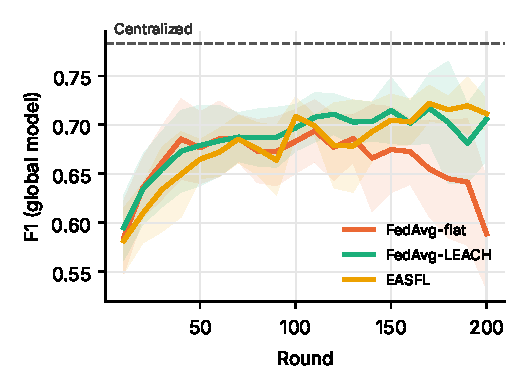
\includegraphics[width=0.65\linewidth]{figs/fig_convergence.pdf}
\caption{F1 of the global model during training (mean $\pm$ std, 5 seeds). FedAvg-flat degrades as its nodes die.}
\label{fig:conv}
\end{figure}

\subsection{Network Lifetime and Ablation}
Fig.~\ref{fig:alive} shows alive nodes over time and Table~\ref{tab:life} the lifetime milestones. EASFL delays the first node death to round 547, against 35 for FedAvg-LEACH (15.6$\times$) and 25 for centralized collection, and its HND (645) is 4.4$\times$ that of FedAvg-LEACH. Its characteristic ``plateau then cliff'' curve reflects balanced drain: no node dies until residual energies have been evened out.

\begin{figure}[t]
\centering
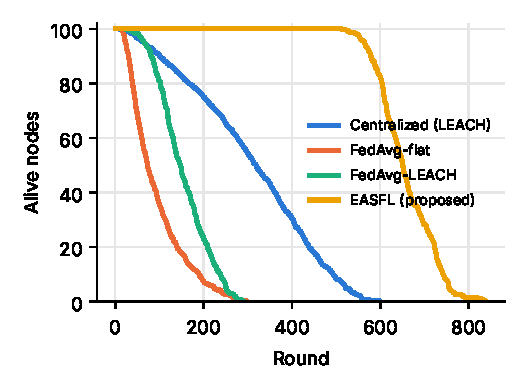
\includegraphics[width=0.65\linewidth]{figs/fig_alive.pdf}
\caption{Alive nodes per round (mean of 5 seeds, 60 raw samples per node-round for centralized collection).}
\label{fig:alive}
\end{figure}

\begin{table}[t]
\caption{Lifetime (Rounds) and Energy in the First 200 Rounds}\label{tab:life}
\centering\footnotesize
\begin{tabular}{@{}lcccc@{}}
\toprule
Scheme / variant & FND & HND & LND & $E_{200}$ (J)\\
\midrule
Centralized (LEACH) & 25 & 320 & 489 & 25.9\\
Centralized (EA-CH) & 142 & 246 & 461 & 39.1\\
FedAvg-flat & 18 & 73 & 189 & 49.0\\
FedAvg-LEACH & 35 & 145 & 233 & 47.3\\
\textbf{EASFL} & \textbf{547} & 645 & 731 & \textbf{15.6}\\
\quad w/o participant selection & 317 & 538 & 628 & 19.4\\
\quad w/o compression & 219 & 248 & 291 & 40.9\\
\quad w/o energy-aware CH (LEACH) & 177 & \textbf{697} & \textbf{802} & 15.9\\
\bottomrule
\end{tabular}
\end{table}

\begin{figure}[t]
\centering
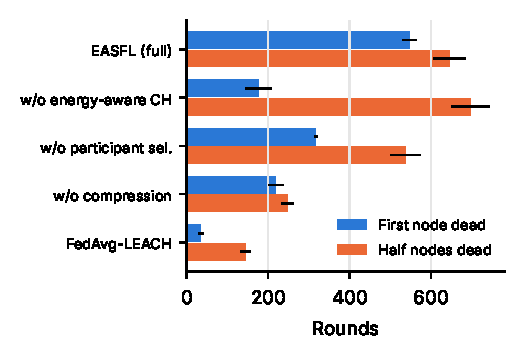
\includegraphics[width=0.65\linewidth]{figs/fig_ablation.pdf}
\caption{Ablation: contribution of each EASFL component to lifetime (mean $\pm$ std).}
\label{fig:abl}
\end{figure}

The ablation (Table~\ref{tab:life}, Fig.~\ref{fig:abl}) isolates each component. Compression is the largest contributor: without it, energy use rises 2.6$\times$ and HND falls from 645 to 248. Participant selection adds 73\% to FND. Energy-aware CH selection triples FND (547 vs.\ 177) but slightly shortens HND and LND relative to LEACH rotation (645 vs.\ 697, 731 vs.\ 802). This is a genuine trade-off: deterministic selection favours nodes close to the BS and well connected, which equalizes early drain but concentrates the CH burden on a subset late in life. Applications that need full coverage (FND) should prefer the energy-aware score; those that tolerate gradual coverage loss may prefer rotation. The same trade-off appears when the energy-aware score is applied to centralized collection (FND 25 $\rightarrow$ 142, HND 320 $\rightarrow$ 246).

\subsection{Robustness to Poisoning}
Fig.~\ref{fig:pois} plots global-model F1 against the fraction of malicious nodes for the four attacks, and Table~\ref{tab:pois} details the 20\% case. Undefended FedAvg collapses under the scaled sign flip (F1 0.24 at 20\%, 0.13 at 30\%). With 10\% and 20\% attackers, EASFL keeps global F1 between 0.64 and 0.71 across all attacks, within 0.07 of its clean value (0.71) and higher than every compared aggregation rule in all eight cases. Removing EASFL's filtering and quarantine (``EASFL w/o robust'') lets the sign-flip attack succeed (0.18), confirming that the defence and not compression or participant selection provides the resilience. The label-flip attack is notable: its updates are neither large nor reversed in direction, yet EASFL (0.67) outperforms median (0.53) and trimmed mean (0.57), because repeated flags quarantine persistent offenders. Krum performs poorly throughout (0.35--0.52), even without attackers, because selecting a single update discards the information carried by heterogeneous nodes.

\begin{figure*}[t]
\centering
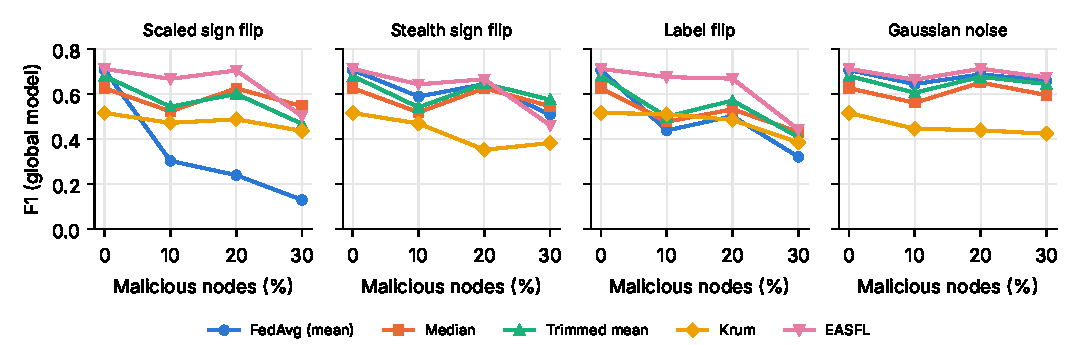
\includegraphics[width=0.95\textwidth]{figs/fig_poisoning.pdf}
\caption{Global-model F1 versus fraction of malicious nodes for four poisoning attacks (mean of 5 seeds).}
\label{fig:pois}
\end{figure*}

\begin{table}[t]
\caption{F1 With 20\% Malicious Nodes: Global Model / Personalized}\label{tab:pois}
\centering\scriptsize
\setlength{\tabcolsep}{3pt}
\begin{tabular}{@{}lcccc@{}}
\toprule
Defence & Sign flip & Stealth & Label flip & Gaussian\\
\midrule
FedAvg (mean) & 0.24 / 0.40 & 0.64 / 0.80 & 0.50 / 0.81 & 0.69 / 0.83\\
Median & 0.62 / 0.81 & 0.63 / 0.81 & 0.53 / 0.82 & 0.65 / 0.82\\
Trimmed mean & 0.60 / 0.80 & 0.65 / 0.81 & 0.57 / 0.82 & 0.68 / 0.83\\
Krum & 0.49 / 0.75 & 0.35 / 0.73 & 0.48 / 0.75 & 0.44 / 0.73\\
EASFL w/o robust & 0.18 / 0.41 & 0.66 / 0.81 & 0.43 / 0.82 & 0.70 / 0.82\\
EASFL w/o cosine & 0.70 / 0.81 & 0.66 / 0.80 & 0.65 / 0.82 & 0.70 / 0.82\\
\textbf{EASFL} & \textbf{0.70} / 0.82 & \textbf{0.67} / 0.81 & \textbf{0.67} / 0.82 & \textbf{0.71} / 0.82\\
\bottomrule
\end{tabular}
\end{table}

Two further observations matter for practice. First, personalization is itself a strong mitigation: after local fine-tuning, label-flip and Gaussian attacks barely affect any scheme. It does not, however, rescue the undefended schemes from the sign-flip attack (0.40), so robust aggregation remains necessary. Second, the defence has limits. At 30\% attackers EASFL becomes unstable across seeds (sign flip: F1 0.50 $\pm$ 0.25; stealth: 0.46 $\pm$ 0.21), whereas the coordinate-wise median degrades more gracefully (0.55 in both cases). We therefore claim resilience up to 20\% compromised nodes. The cosine test added little beyond the norm test and quarantine (Table~\ref{tab:pois}); it is cheap and retained, but its effect is not statistically distinguishable in our runs.

\subsection{Packet Loss}
With packet-loss probabilities from 0 to 0.3, EASFL's global F1 stays between 0.69 and 0.72 and its personalized F1 at 0.82, whereas FedAvg-LEACH's global F1 falls from 0.69 to 0.65 at 30\% loss. Because each round aggregates many small, independent uploads, isolated losses mainly reduce the effective participation rather than biasing the update.

\subsection{Sensitivity to the Synthetic Workload}
To verify that the conclusions are not artefacts of the generator settings, we varied the Dirichlet concentration $\alpha\in\{0.1,\dots,10\}$, the fault magnitude ($0.5$--$1.5\times$) and the anomaly rate ($0.5$--$2\times$). Fig.~\ref{fig:sens} shows that personalized EASFL matches or exceeds the centralized model in every setting except the smallest faults ($0.5\times$, where all methods reach only F1 $\approx0.54$ because faults are within noise), and stays within 0.02 of personalized FedAvg-LEACH throughout. Energy and traffic do not depend on the data, so EASFL's lifetime advantage is unaffected by these settings.

\begin{figure*}[t]
\centering
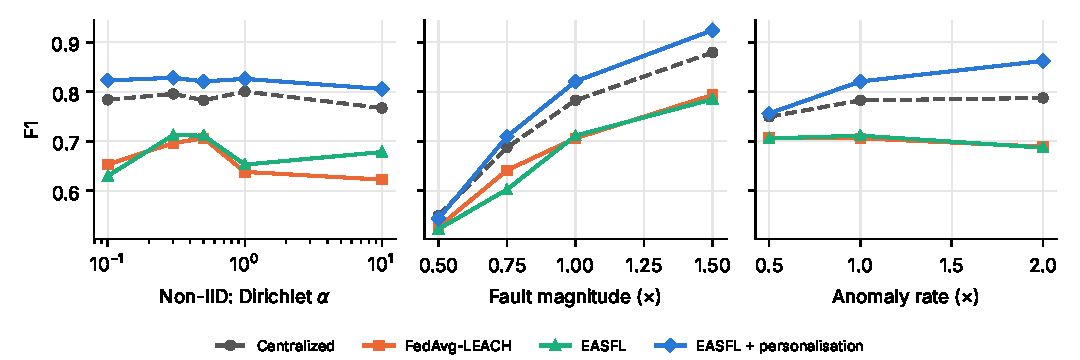
\includegraphics[width=0.95\textwidth]{figs/fig_sensitivity.pdf}
\caption{Sensitivity of F1 to the non-IID degree (Dirichlet $\alpha$), fault magnitude and anomaly rate (mean of 5 seeds).}
\label{fig:sens}
\end{figure*}

\subsection{When Is Centralized Collection Preferable?}
The energy of centralized collection grows with the raw sampling volume, whereas EASFL's communication does not. Varying the samples each node reports per round, centralized collection with LEACH achieves FND/HND of 81/1379 rounds at 10 samples, 45/589 at 30, 25/320 at 60 and 6/85 at 240. Hence, for very low reporting rates ($\le$10 samples per round) centralized collection outlives EASFL in HND, although its FND remains far shorter (81 vs.\ 547); above roughly 30 samples per round EASFL dominates on all lifetime metrics. The model size and the sampling rate together determine which design is preferable, and the cost model of Section~\ref{sec:model} allows this crossover to be computed before deployment.

\section{Discussion and Limitations}
\textit{Synthetic data.} The workload is synthetic by design, which provides exact ground truth and controllable heterogeneity, and we mitigate the risk of generator artefacts with the sensitivity analysis above. Absolute F1 values depend on the fault model; the relative conclusions (comparable per-node accuracy, large lifetime and network-level gains, resilience up to 20\%) are consistent across all settings tested. Validation on deployment traces with expert labels is a natural next step.

\textit{Simulator scope.} The round-based simulator abstracts MAC contention, retransmissions, idle listening and sleep scheduling, which affect all schemes but may change absolute lifetimes. Training energy uses a fixed per-sample cost; on microcontrollers without floating-point units this cost can be higher, which would favour EASFL's participant selection further.

\textit{Threat model.} We assume honest CHs and non-colluding, non-adaptive attackers. Adaptive attacks crafted against the specific defence~\cite{fang2020}, backdoors~\cite{bagdasaryan2020} and compromised CHs remain open. EASFL provides integrity protection, not confidentiality; it can be combined with secure aggregation~\cite{bonawitz2017} at the cost of extra communication.

\section{Conclusion}
EASFL shows that federated anomaly detection can extend, rather than shorten, the life of a WSN when every protocol component is designed around radio energy. Compressed, selectively scheduled updates cut traffic by $13\times$ and energy by $3\times$ relative to hierarchical FedAvg and postpone the first node death by more than an order of magnitude; on-node personalization lifts per-node F1 above that of a centralized model without any radio cost; and two-tier robust aggregation with quarantine maintains accuracy with up to 20\% malicious nodes. Measured at the network level, where dead nodes cannot report anomalies, EASFL detects anomalies with F1 0.82 at round 200 while hierarchical FedAvg reaches 0.26. Future work will validate EASFL on real deployment traces, extend the threat model to adaptive attackers and compromised CHs, and explore adaptive participation ratios driven by energy harvesting.

\section*{Code Availability}
The simulator, experiment scripts, random seeds and raw results are available at \url{https://github.com/vadlashiva/EASFL}.

\bibliographystyle{IEEEtran}
\bibliography{refs}

\end{document}
